\subsubsection{Hardware}

Ursprünglich war geplant eine Varaiante des Turms mit 40 Stellplätzen zu bauen. Wengen Zeitmangel wurde die Anzahl der Stellplätze auf 8 reduziert. Zusätzlich wurde nur die vordere Hälfte des Turms gebaut.

\paragraph{Stückliste (Reduzierte Version):}
\begin{itemize}
  \item 1x \textbf{Raspberry Pi 4b}: Hauptplatine des Turms.
  \item 8x \textbf{5mm Neopixel RGB Throughhole LEDs}: LEDs für die Anzeige der Boxen.
  \item 4x \textbf{3D-Druck Turmsegment}: Einzelne Segmente des Turm Modells.
\end{itemize}

\paragraph{Stückliste (Vollständige Version):}
\begin{itemize}
  \item 1x \textbf{Raspberry Pi 4b}
  \item 20x \textbf{5mm Neopixel RGB Throughhole LEDs}
  \item 20x \textbf{3D-Druck Turmsegment}
\end{itemize}

\paragraph{Elektronik}

Das folgende Ersatzschaltbild zeigt die Verkabelung des Turms. Die LEDs werden über den GPIO Port des Raspberry Pi angesprochen. Die Ansteuerung der LEDs erfolgt über die \texttt{Neopixel} Bibliothek. Die Datenleitungen der LEDs sind in Serie geschaltet. Die Stromversorgung der LEDs erfolgt über den 5V Port des Raspberry Pi. Die Stromversorgung des Raspberry Pi erfolgt über das mitgelieferte Raspberry Pi Netzteil.

\begin{figure}[H]
  \centering
  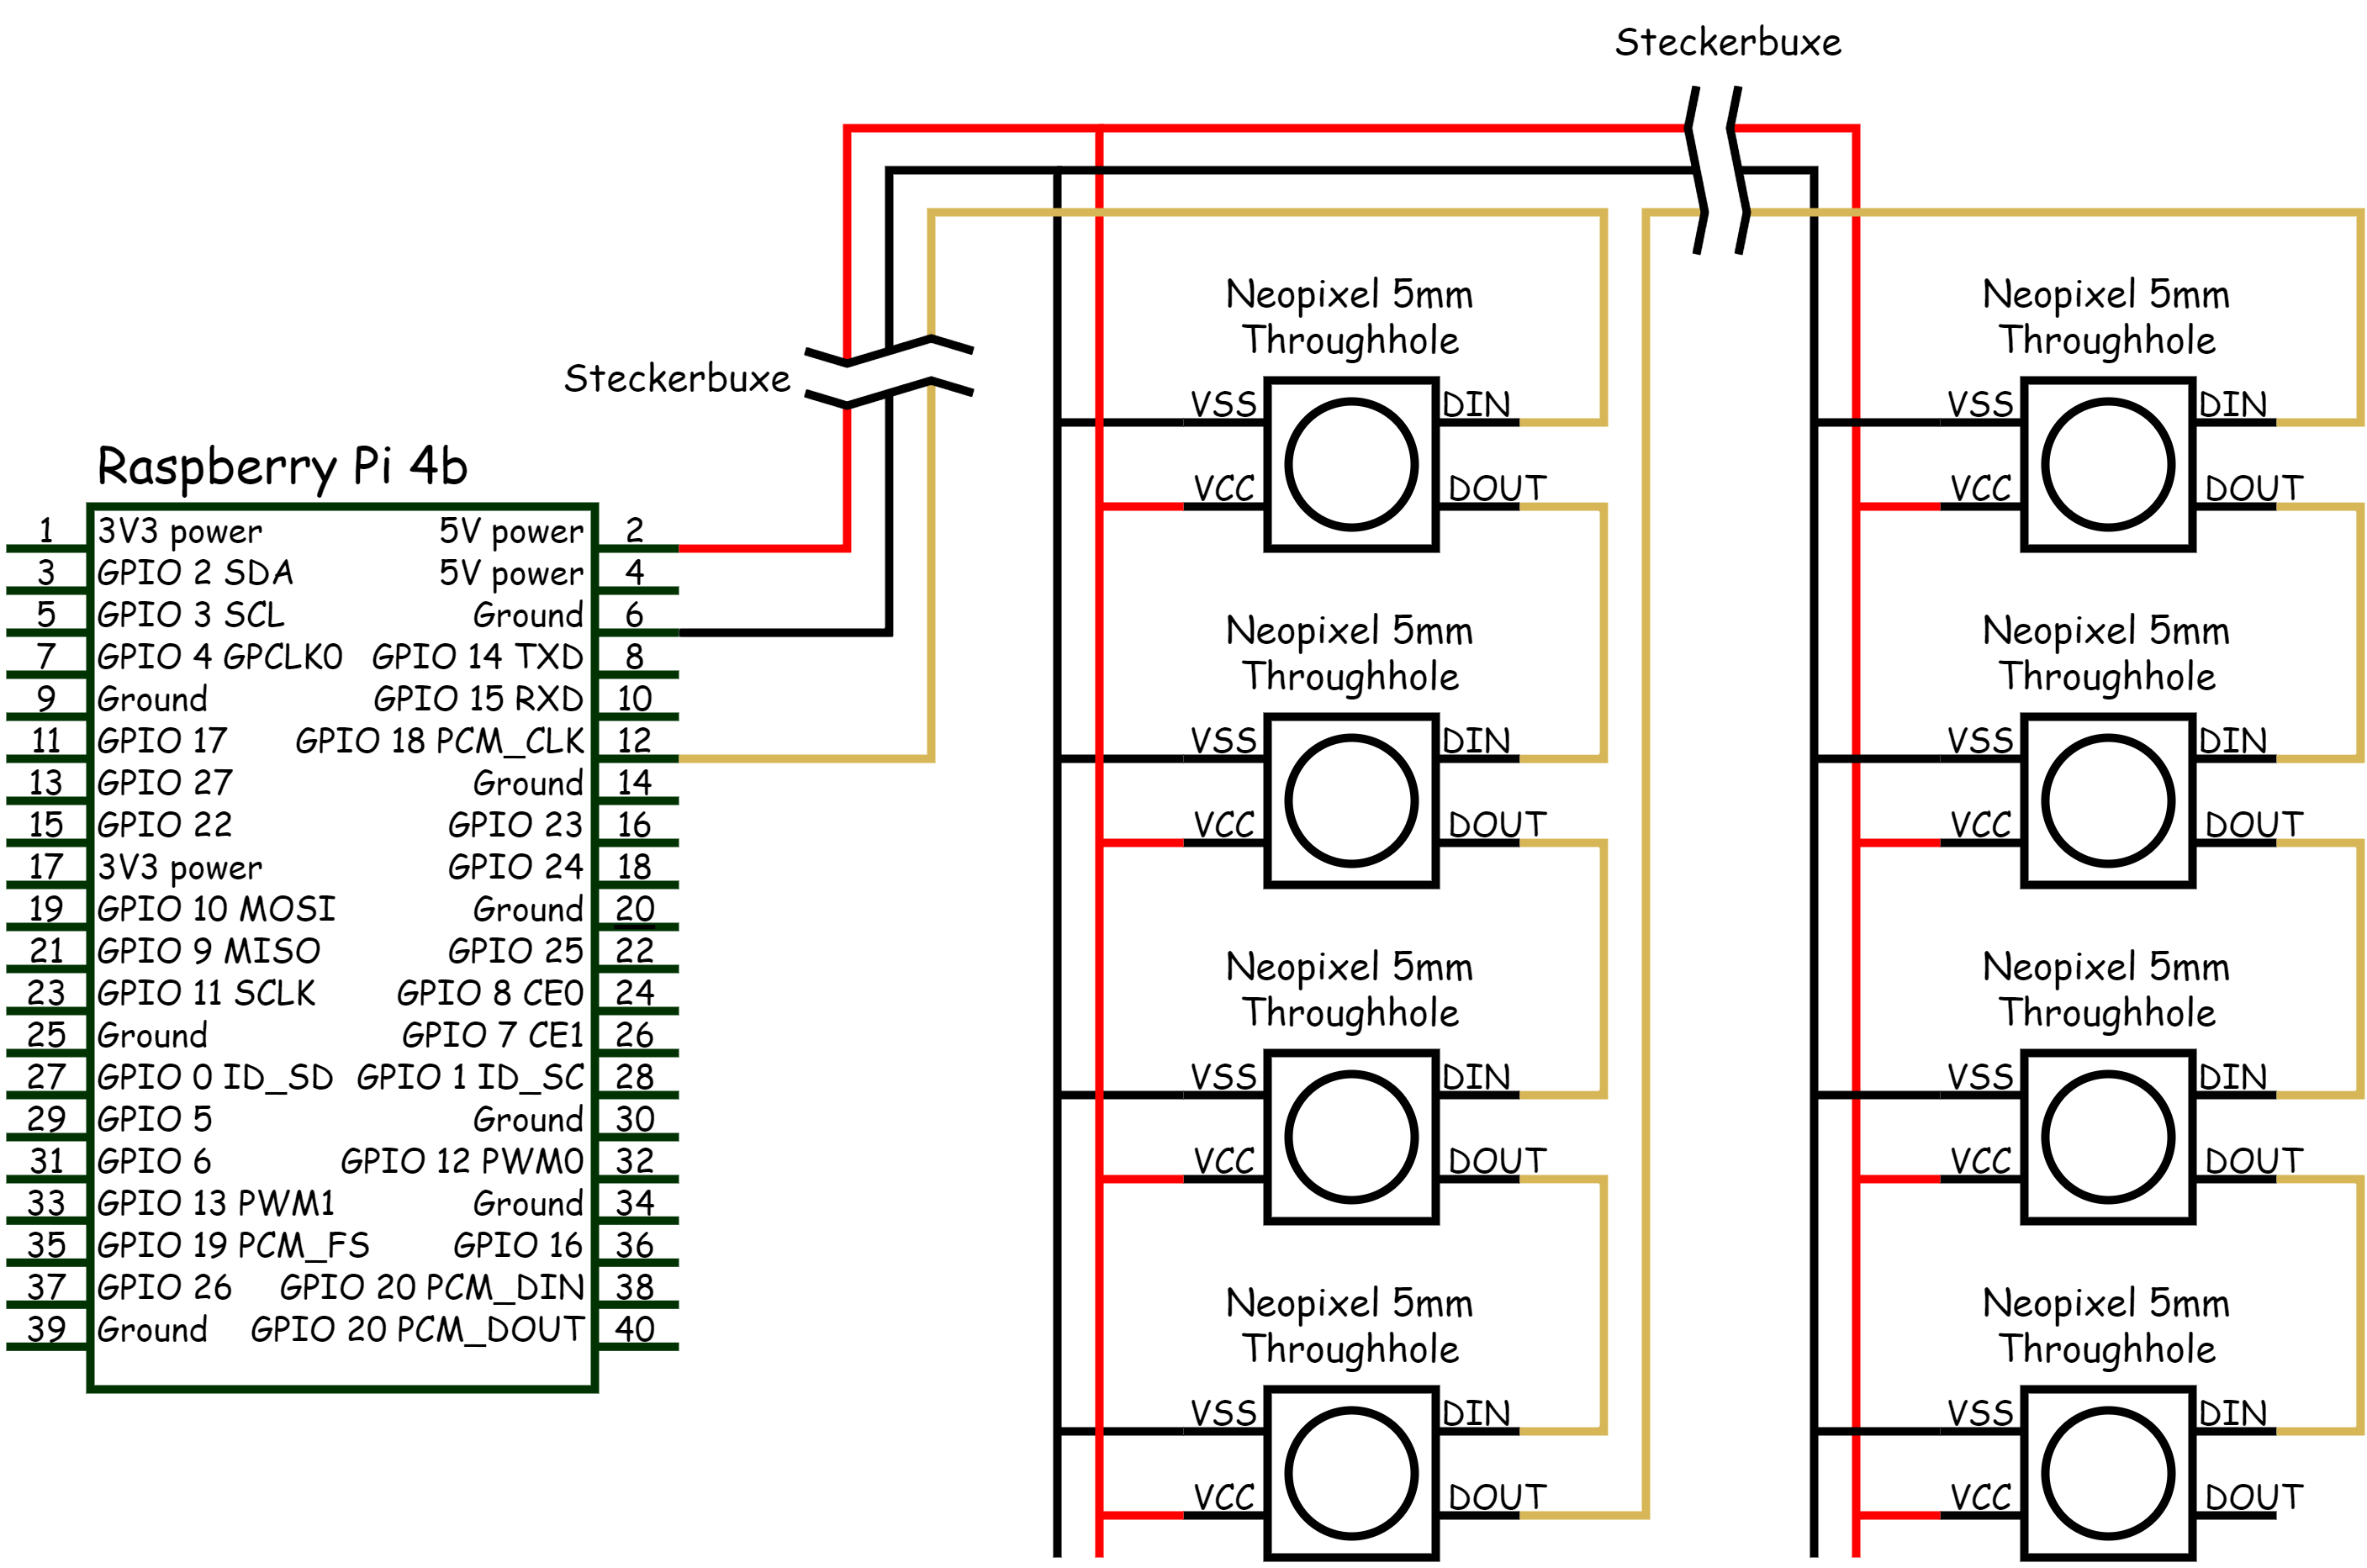
\includegraphics[width=0.75\textwidth]{images/tower_controller_v4_circuit_diagram.png}
  \caption{Ersatzschaltbild des Turms}
  \label{fig:ersatzschaltbild}
\end{figure}

Die einzelnen Komponenten wurden mittels eines Lötkolben verlötet. Jede Ebene des Turmes wurde einzeln verlötet, sodass die einzelnen Ebenen des Turmes später einfach zusammengesteckt werden können.

\paragraph{3D-Druck}

Die eigentliche Form des Turm Models wurde mit dem 3D-Drucker gedruckt. Dazu wurde das Miniaturmodell zuerst in Autodesk Inventor konstruiert \ref{fig:modell_segment}. Anschließend wurde dies als STL-Datei exportiert und in SuperSlicer für den 3D-Druck vorbereitet. Da die Zeit sehr Knapp war, wurden die Druckparameter so gewählt, dass der Druck möglichst schnell fertig wurde. Die Druckparameter sind in Tabelle \ref{tab:druckparameter} aufgeführt. Der Gcode wurde Exportiert und mittels Octoprint auf einem Wanhao i3 Drucker ausgeführt. Die finale Druckzeit pro Teil betrug ca. 10 Stunden.